As the behaviour of each individual agent has been described and tested, the next step is looking at a market consisting of some or all of the agents. This has been described in both Oesch 2014 \cite{Oesch} and McG \cite{McGroarty} papers. By comparing the results produced, one can confirm that the agents have been correctly implemented. 


\section{Oesch's Experiment configuration compared to McG}
McG claims that they have taken the Liquidity consumer and Market maker (Liquidity provider) from the Oesch paper. In addition, both papers referred to Wei and Barbazon \cite{CuiNoise} in Noise trader algorithm. Oesch provides an example result of running the three agents in the same market in addition to the mid price and return series graph. This is a great benchmark to compare whether the agents' behaviour is correct. If the results are similar, it can be concluded that at least three out of five agents are acting correctly when McG results are compared. 

However, Oesch's time-steps are different than that of McG's and very similar to the BSE. In each time-step, the system will randomly select one group of agent based on a probability and then select an agent to act in that time-step. The system is more sequential where one agent can only act in a time-step. This means that we have to adapt the Oesch time-step into the McG time-step. We chose 10,000 action steps of the McG which is more than Oesch, but through multiple experiment, is required to show the price patterns. This allows the market itself to run for a period of time in order to exhibit the market behaviour for each configuration but is less than the original McG time-step since Oesch ran their experiment in a shorter time-period.

In our initial results, we were able to replicate similar price movements with Oesch's time-steps with McG version of Liquidity consumer, Market maker and Noise trader. We will be comparing the \textbf{Mid-Price} or the average price between best Ask price and best Bid price given by: 
\begin{equation}
    Mid Price = (BestAskPrice + BestBidPrice) / 2
\end{equation}

\begin{figure}[h]
  \begin{subfigure}[b]{0.5\textwidth}
    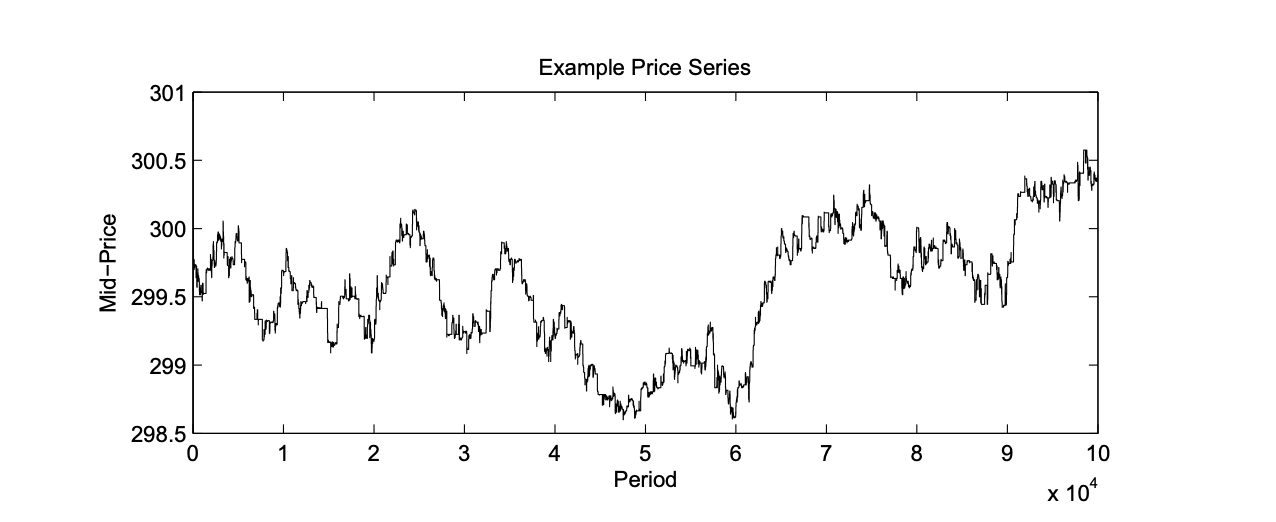
\includegraphics[width=8cm, height=8cm]{Dissertation/images/Market_experiment/Original_mp.png}
    \caption{Original Mid Price \cite{Oesch}}
    \label{fig:O_original_mp}
  \end{subfigure}
  %
  \begin{subfigure}[b]{0.5\textwidth}
    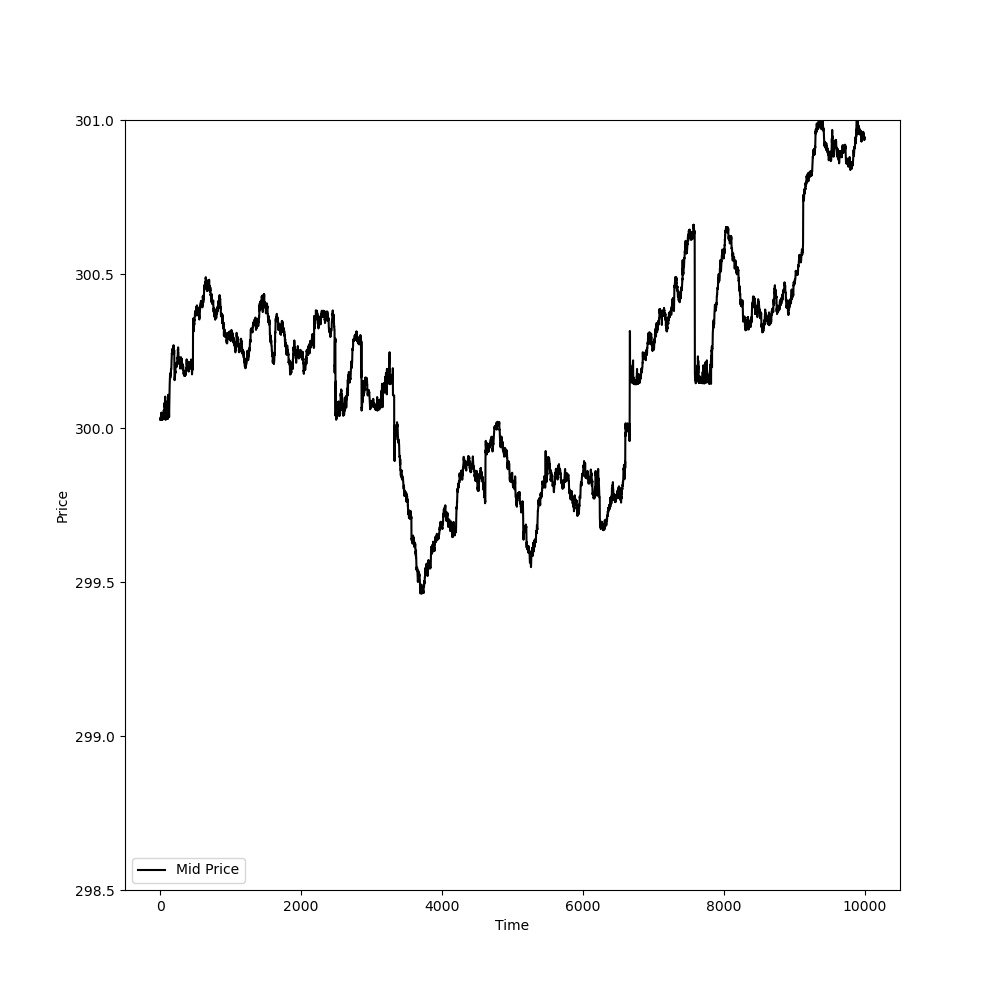
\includegraphics[width=8cm, height=8cm]{Dissertation/images/Market_experiment/282826.png}
    \caption{Experiment Mid price Series}
    \label{fig:O_experiment_mp}
  \end{subfigure}
\caption{Mid Price series: Replication of Oesch's experiments with similar configurations in a market with 56 Liquidity consumer, 56 Market maker and 52 Noise traders} 
\label{fig:Oesch_mp}
\end{figure}

\begin{figure}[h]
  \begin{subfigure}[b]{0.5\textwidth}
    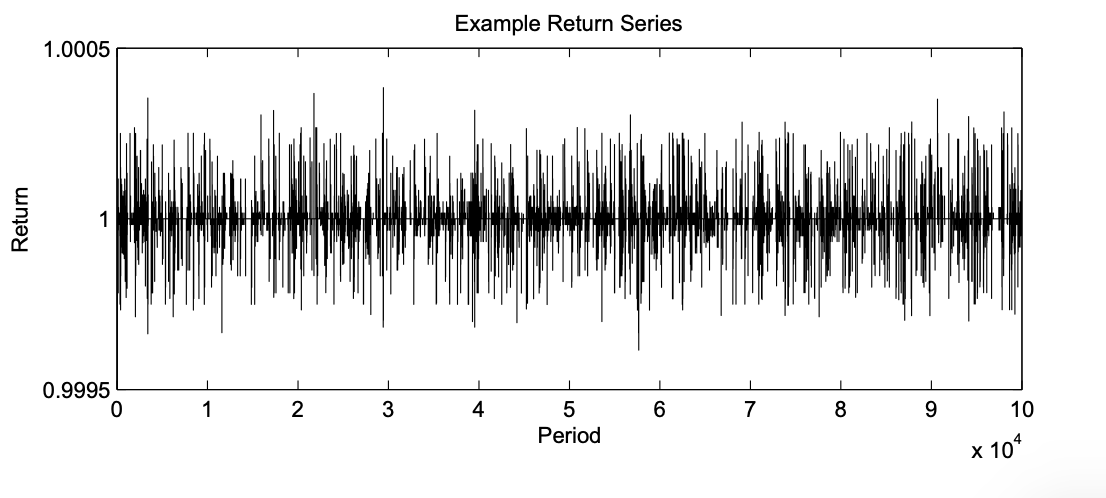
\includegraphics[width=8cm, height=7cm]{Dissertation/images/Market_experiment/Original_return.png}
    \caption{Original Return Series \cite{Oesch}}
    \label{fig:O_original_return}
  \end{subfigure}
  %
  \begin{subfigure}[b]{0.5\textwidth}
    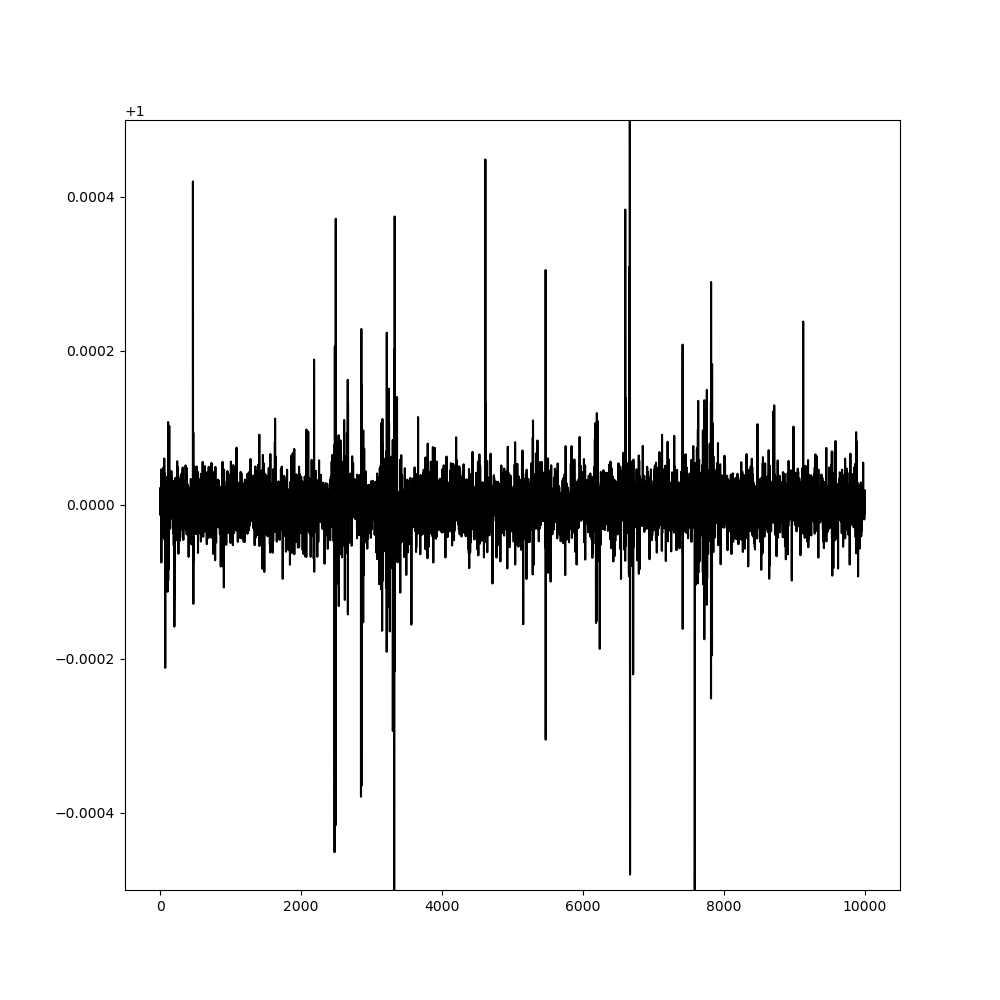
\includegraphics[width=8cm, height=7cm]{Dissertation/images/Market_experiment/282826-r.png}
    \caption{Experiment Return Series}
    \label{fig:O_experiment_return}
  \end{subfigure}
\caption{Return series: Replication of Oesch's experiments with similar configurations in a market with 56 Liquidity consumer, 56 Market maker and 52 Noise traders } 
\label{fig:Oesch_return}
\end{figure}
\FloatBarrier

Figure \ref{fig:Oesch_mp} and \ref{fig:Oesch_return} illustrate the results after replication of Oesch's experiment. The market consists of 56 Market maker, 56 Liquidity consumer and 52 Noise traders. These numbers will be explained in more detailed and explored more clearly in the next subsections. The mid price value is still in range of the original experiment, which is between 298.5 and 301. The price movement exhibits similar movements over the period of time. However, the return series are not the same even though they are in the same range. There are some important factors that contribute to why the results may not be totally similar. 

\begin{itemize}
  \item Oesch's results in mid price and return series does not state how many or what is the ratio of the agent types in the market when the experiment is being conducted.
  \item The details of the agents are all explained with only words with no psuedocode, which may not be as detailed as the one described in McG with clear algorithm. McG does not state that the agents are replicated, but rather "modelled after". There are obvious difference between the agents in the two papers and the difference in results can be correlated with the missing details of the agents in Oesch's. 
\end{itemize}

\section{Number of agents and effect on the market}

One interesting trend is that as the number of agents in the market increases, the smaller the range of the return series will be. This means that the change in mid-price in each action step is less than before. The pattern emerged from the fact that since there are more Liquidity consumer and Market maker, there are more orders around the same price range since both of these agents submit only a market order and limit order at the best price. This means that there is more liquidity in the market which can produce smaller returns. In addition, because the Noise agent will submit mostly an "off-spread" price, which is lower/higher than the best bid/ask price, the best bid and ask orders will be executed first. 

\begin{figure}[h]
  \begin{subfigure}[b]{0.5\textwidth}
    \includegraphics[width=7cm, height=7cm]{Dissertation/images/Market_experiment/different_num_agents/202020.png}
    \caption{40 of each agent}
    \label{fig:1}
  \end{subfigure}
  %
  \begin{subfigure}[b]{0.5\textwidth}
    \includegraphics[width= 7cm, height= 7cm]{Dissertation/images/Market_experiment/different_num_agents/303030.png}
    \caption{60 of each agent}
    \label{fig:2}
  \end{subfigure}

  \begin{subfigure}[b]{0.5\textwidth}
    \includegraphics[width=7cm, height=7cm]{Dissertation/images/Market_experiment/different_num_agents/404040.png}
    \caption{80 of each agent}
    \label{fig:1}
  \end{subfigure}
  %
  \begin{subfigure}[b]{0.5\textwidth}
    \includegraphics[width= 7cm, height=7cm]{Dissertation/images/Market_experiment/different_num_agents/505050.png}
    \caption{100 of each agent}
    \label{fig:2}
  \end{subfigure}
\caption{Return Series of different number of agents in the market ran with 10,000 McG action steps} 
\end{figure}
\FloatBarrier

\section{The effect of number of agents on Mid-price patterns}

In this section, we will explore the pattern of the price series when there are different number of agents in the market. The market is ran with 10,000 action steps where different number of agents are present in the market with initial price of 300. There are three agents in the market : Liquidity consumer, Market maker and Noise trader. 

\begin{figure}[h]
  \begin{subfigure}[b]{0.5\textwidth}
    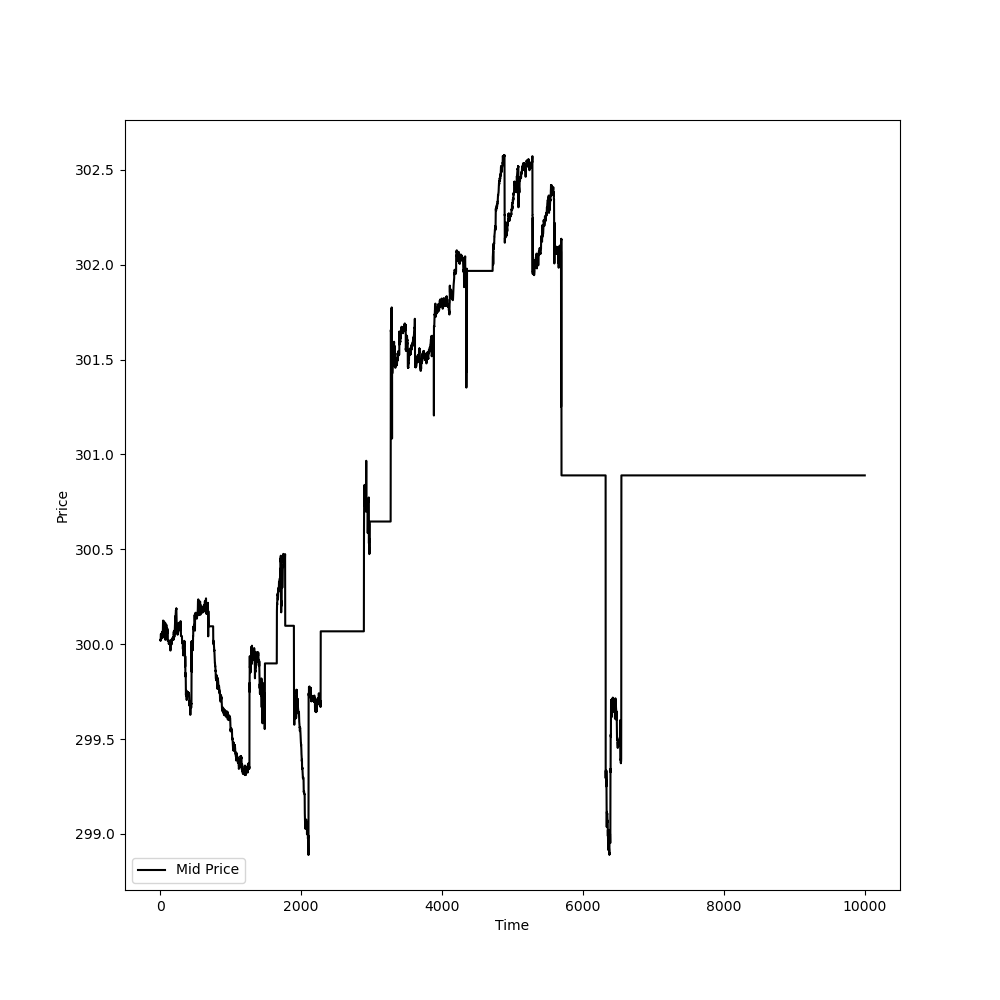
\includegraphics[width=7cm, height=7cm]{Dissertation/images/Market_experiment/oscil_num/151515.png}
    \caption{30 of each agent}
    \label{fig:O_experiment_30}
  \end{subfigure}
  %
  \begin{subfigure}[b]{0.5\textwidth}
    \includegraphics[width= 7cm, height= 7cm]{Dissertation/images/Market_experiment/oscil_num/202020.png}
    \caption{40 of each agent}
    \label{fig:O_experiment_40}
  \end{subfigure}

  \begin{subfigure}[b]{0.5\textwidth}
    \includegraphics[width=7cm, height=7cm]{Dissertation/images/Market_experiment/oscil_num/303030.png}   \caption{60 of each agent}
    \label{fig:O_experiment_60}
  \end{subfigure}
  %
  \begin{subfigure}[b]{0.5\textwidth}
    \includegraphics[width= 7cm, height= 7cm]{Dissertation/images/Market_experiment/oscil_num/404040.png}
    \caption{80 of each agent}
    \label{fig:O_experiment_80}
  \end{subfigure}

  \begin{subfigure}[b]{0.5\textwidth}
    \includegraphics[width=7cm, height=7cm]{Dissertation/images/Market_experiment/oscil_num/505050.png}
    \caption{100 of each agent}
    \label{fig:O_experiment_100}
  \end{subfigure}
  %
  \begin{subfigure}[b]{0.5\textwidth}
    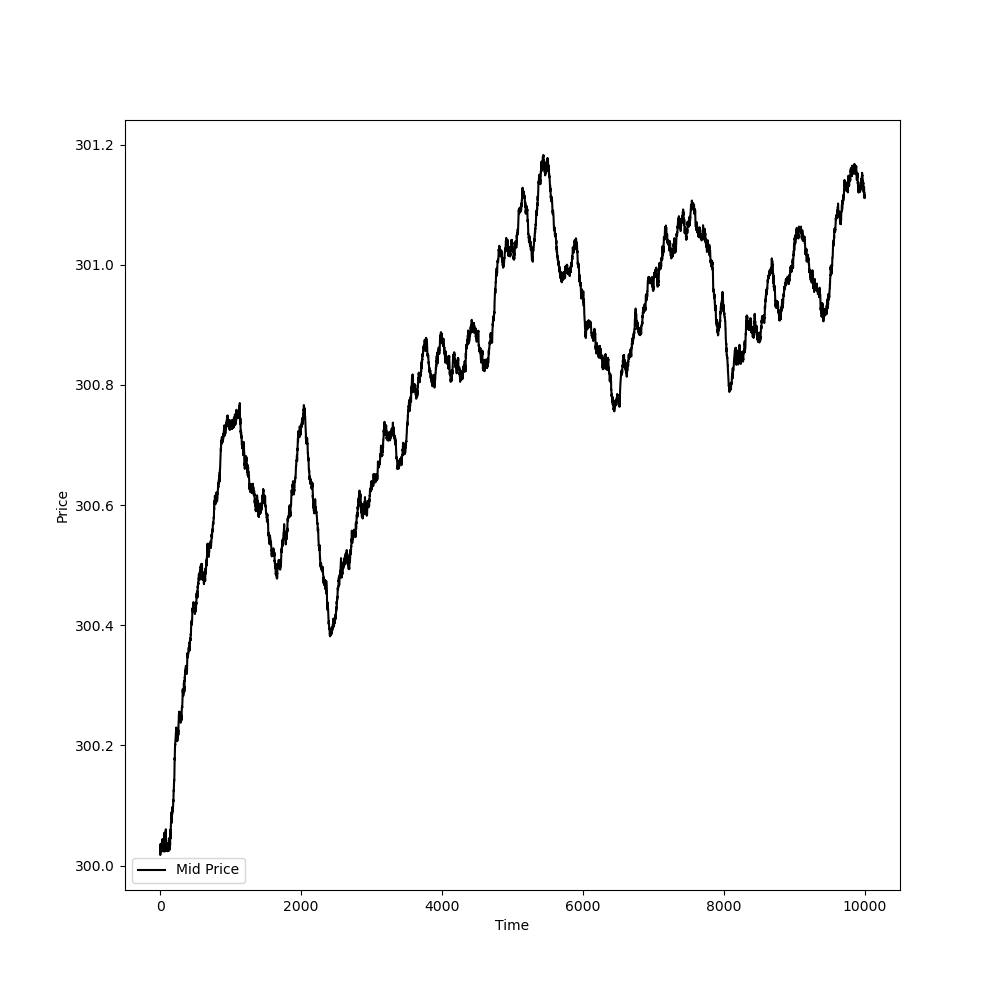
\includegraphics[width= 7cm, height=7cm]{Dissertation/images/Market_experiment/oscil_num/606060.png}
    \caption{120 of each agent}
    \label{fig:O_experiment_120}
  \end{subfigure}
\caption{Mid price Series of different number of agents in the market} 
\end{figure}
\FloatBarrier

There are a few pattern worth noting from these figures: 
\begin{itemize}
  \item \textbf{The lower the number of agents, the more unrealistic price patterns will emerge : } It is can clearly be seen in Figure \ref{fig:O_experiment_30} and \ref{fig:O_experiment_40} that there are periods in the experiment where there are huge price spike and periods where price does not change at all, which is unrealistic. This can happen from a number of reasons. First, because we have less Market maker in these market, the orders submitted from each individual Market maker will be executed more quickly, making it submit more large orders, thus more ``spikes" in the price due to large orders. Secondly, because there are  orders submitted to the LOB, in each action-step, all of the orders will be matched, therefore keeping the mid price stable. It can clearly be seen that in Figure \ref{fig:O_experiment_30} there is more of these stable periods than Figure \ref{fig:O_experiment_40}. However, this also means that when Market makers submit a large quantity, it may shift the mid price. 
  
    \begin{figure}[h]
    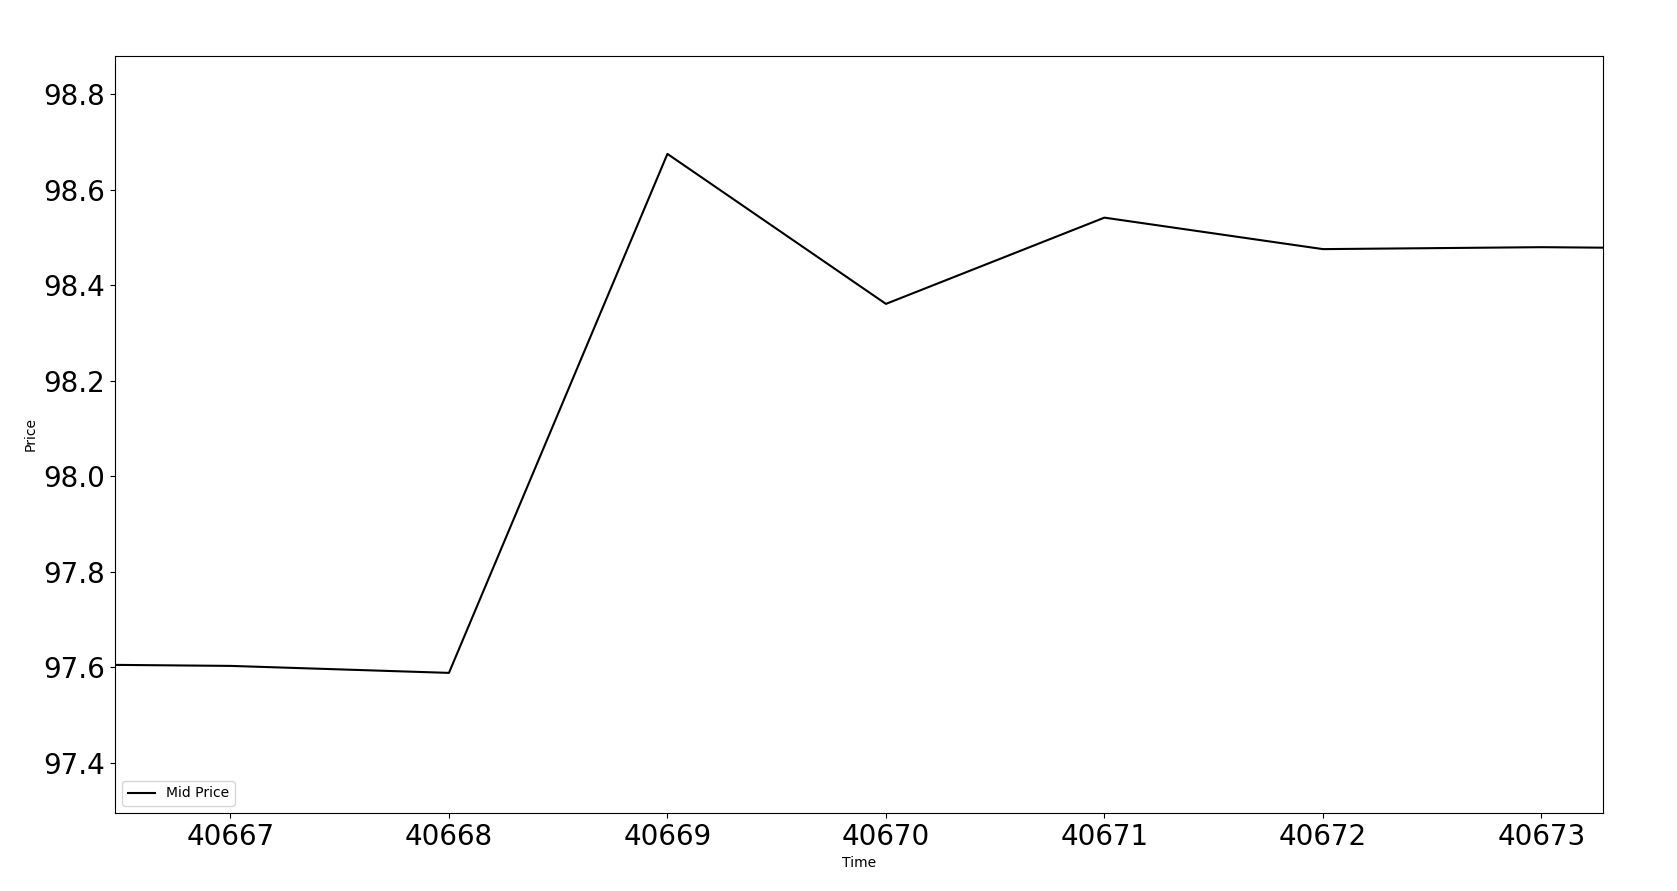
\includegraphics[ height=8cm]{Dissertation/images/Market_experiment/Maket Maker.PNG}
    \caption{Price Spike from Market Maker submitting large order }  
    \label{fig:MM_large}
    \end{figure} 
    \FloatBarrier
  An example of when an order from the Market maker can create a spike in price of the market can be see in Figure \ref{fig:MM_large}. The market is stable in until $t=40668$, where a Market maker submits a large Bid order of quantity 165,000 with shifts the mid price up from 97.6 to 98.6. Because there is now Bid orders left in the order book, the Noise agent responded in $t=40669$ where it submits Ask orders which shift the price down to 98.4. 
  
  \newline Lastly, because these Noise agents are submitting ``off-spread" price in most of the cases and with less of these agents there are in the market, this makes the shift in price more significant since Liquidity consumer's large market orders will execute at any given price in addition to there are no less Noise agents contributing to the change in price. 
  
  \item \textbf{As the number of agents increase, the less likely it will cross the initial mid price : } This is heavily correlated with the pattern seen in Section 5.1.2 with the return series of the mid-price. First, because there are more Noise-traders, this means that the changes in price of the off-spread from each individual agents will be less significant to the market, which means that there are less unrealistic price spikes compared to Figure \ref{fig:O_experiment_30} and Figure \ref{fig:O_experiment_40} where there are less number of agents. In addition, because Market maker only submits at best-price and Liquidity consumer only submitting a market order, the price will move in one direction since for every large order submitted, there is another large order in the opposite side of the book to be matched. It can clearly be seen that in Figure \ref{fig:O_experiment_100} and \ref{fig:O_experiment_120} where the price does not cross in the initial price of 300 at all but rather move in one direction with minor oscillations in between. 
\end{itemize}

\section{Noise agent ratio and its effect on the mid-price pattern} 
This section will explore how the ratio of the Noise agent compared to the market maker and liquidity consumer, more specifically when there are less Noise agents in the market than the other two agents and how we arrived at the final configuration of the Oesch's replicated experiment. The experiment ran with 10,000 action steps with 56 Market maker and Liquidity consumer. This number is from experimenting with 50-60 Market maker and Liquidity consumer since the oscillation is near what is expected from the original paper as experimented in Section 5.2 and 5.3. In addition, from these experiments, these are the maximum number of agents in the market where the price still crosses the initial mid price on average, which is a larger concern than the return series. The figures below illustrate 40 to 55 number of Noise traders. 

\begin{figure}[h]
  \begin{subfigure}[b]{0.5\textwidth}
    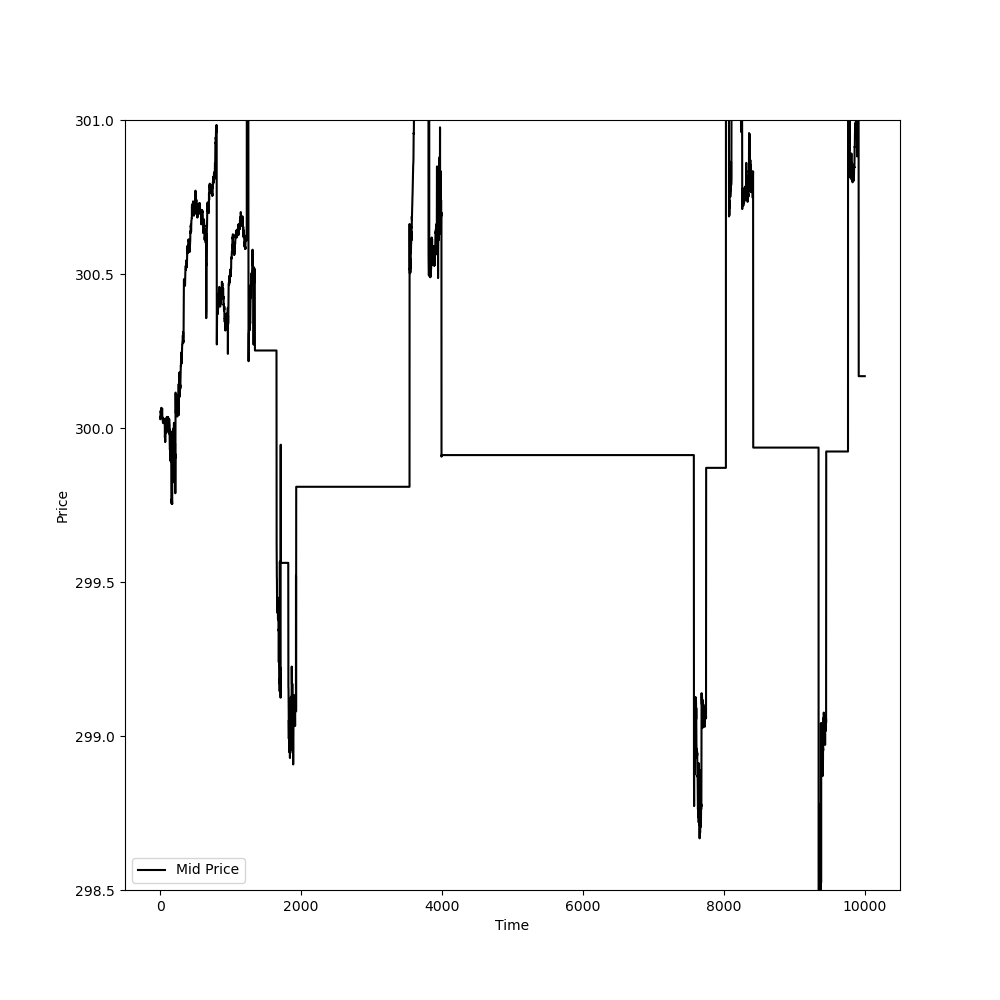
\includegraphics[width=7cm, height=7cm]{Dissertation/images/Market_experiment/ratio/282820.png}
    \caption{40 of Noise traders}
    \label{fig:1}
  \end{subfigure}
  %
  \begin{subfigure}[b]{0.5\textwidth}
    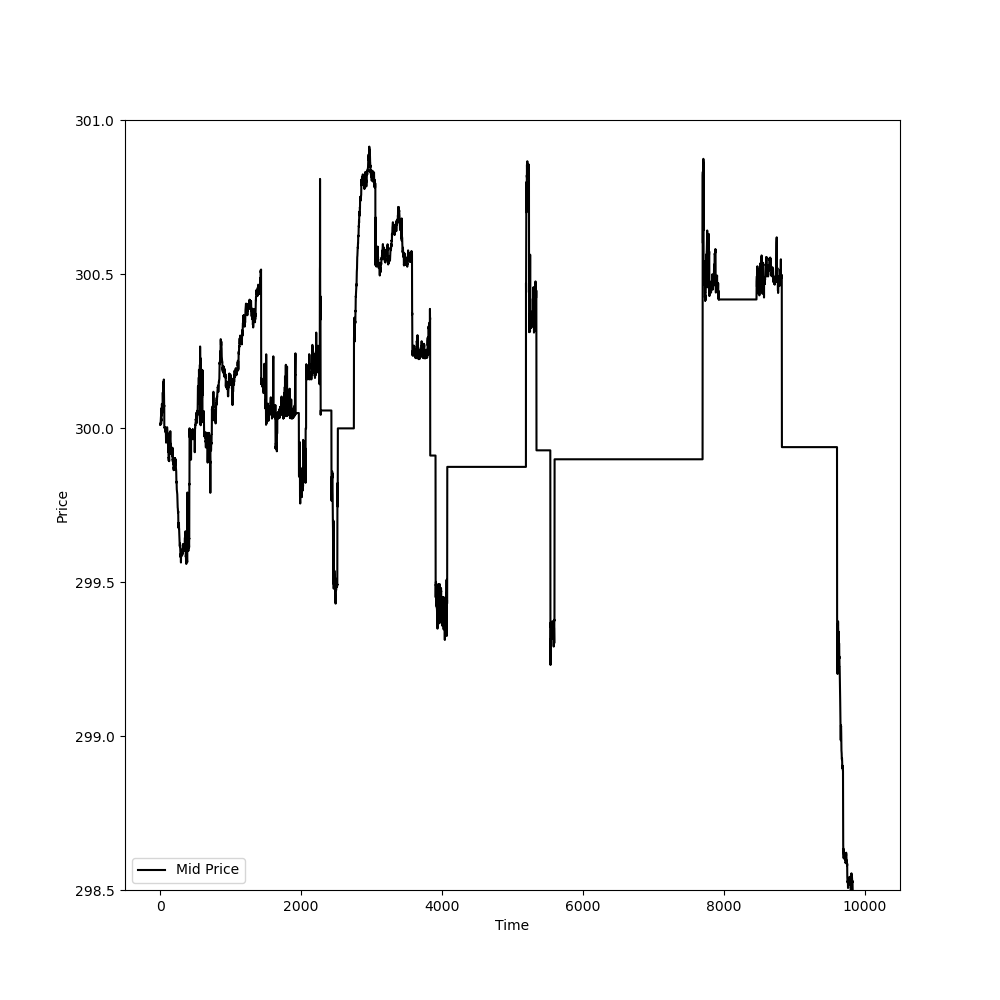
\includegraphics[width= 7cm, height= 7cm]{Dissertation/images/Market_experiment/ratio/282823.png}
    \caption{45 of  Noise traders}
    \label{fig:2}
  \end{subfigure}

  \begin{subfigure}[b]{0.5\textwidth}
    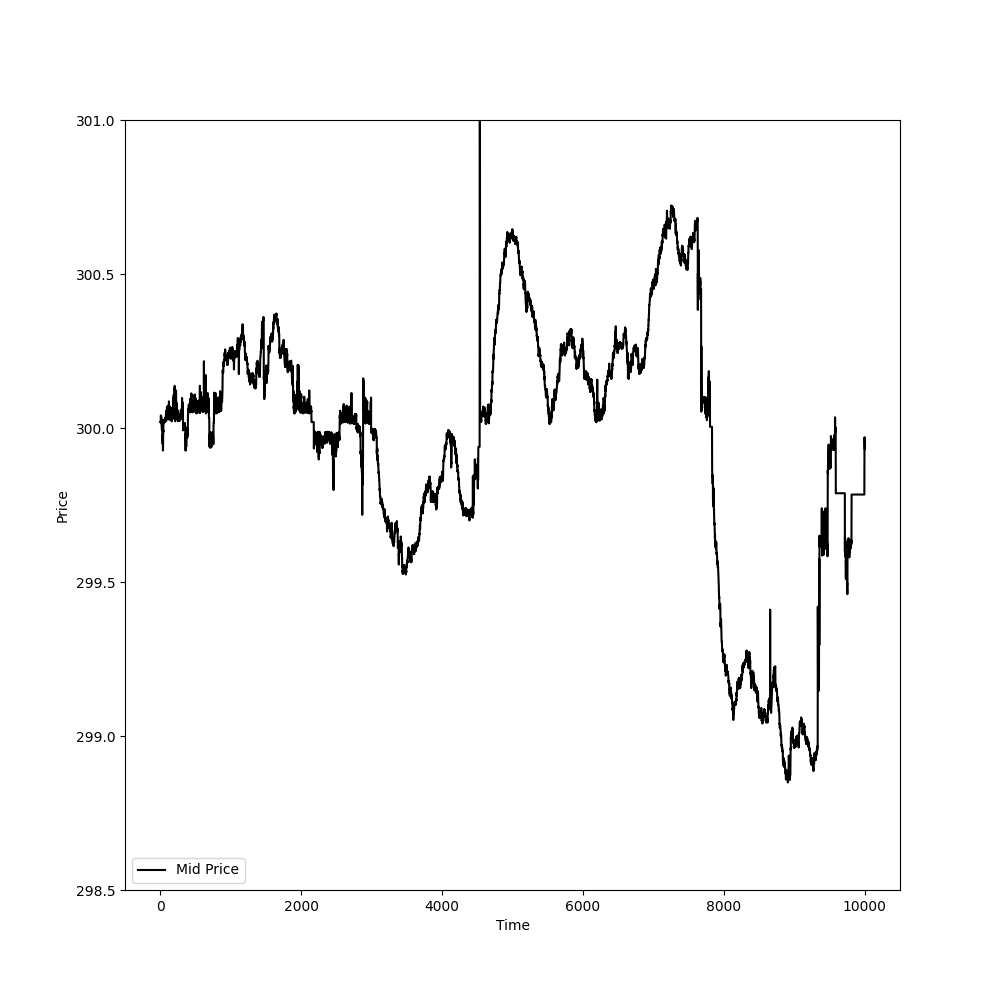
\includegraphics[width=7cm, height=7cm]{Dissertation/images/Market_experiment/ratio/282825.png}   \caption{50 of Noise traders}
    \label{fig:1}
  \end{subfigure}
  %
  \begin{subfigure}[b]{0.5\textwidth}
    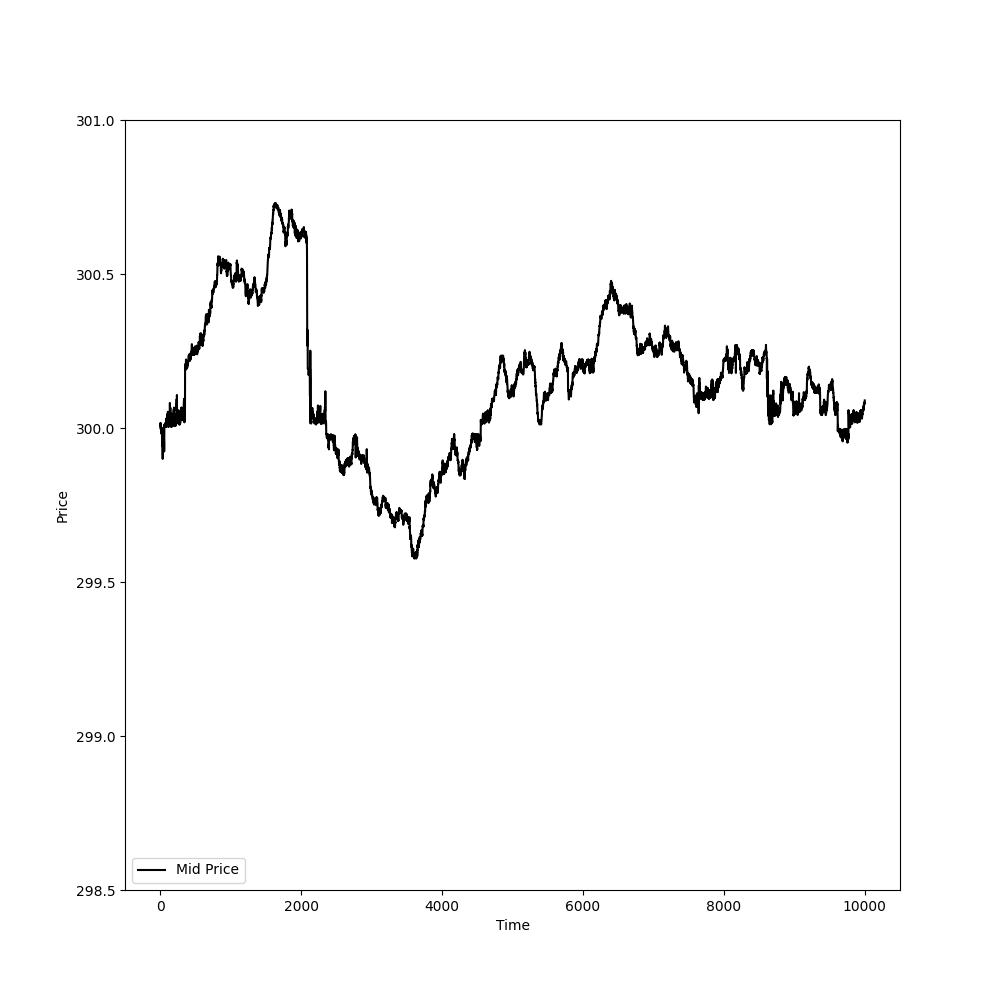
\includegraphics[width= 7cm, height= 7cm]{Dissertation/images/Market_experiment/ratio/282828.png}
    \caption{55 of Noise traders}
    \label{fig:2}
  \end{subfigure}
 \caption{Mid Price Series of different ratio of Noise traders in a market with 56 Liquidity consumer and 56 Market maker} 
\end{figure}
\FloatBarrier

The observation matches what is expected from section 5.1.3 Because there are less Noise agents, the more unrealistic price patterns are observed. This is due to the fact that the contribution of each Noise agent is larger when there are less of them in the market. Another interesting observation from the experiment is that this does not happen when there are roughly equal number of Noise agents than the other two trader types.
